\section{Method}
\label{sec:method}

ICD and AICD share a common construction.  Given a training image and the
classifier in its current state, we compute a saliency map, reduce it to a grid
of tile scores, threshold those scores to obtain a binary mask, and replace the
masked tiles with a fill.  The two methods differ only in the direction of the
threshold.  We describe each step in turn.

\subsection{Saliency Map}
\label{sec:method:saliency}

Let $f_\theta : \mathcal{X} \to \R^{C}$ be a classifier with parameters
$\theta$ over $C$ classes, and let $l$ index a chosen convolutional layer with
feature maps $A^{k,l} \in \R^{h_l \times w_l}$, $k = 1,\dots,K_l$.  Each image
carries a target class $y$ at which the saliency is computed; by default $y$ is
the ground-truth label of the training image, though the model's prediction
$\argmax_c f_\theta(x)_c$ may be substituted.  For an input
$x \in \R^{H \times W \times 3}$ the GradCAM~\citep{selvaraju2017gradcam}
saliency map is
\begin{equation}
  S_\theta(x,y)
  \;=\;
  \mathrm{ReLU}\!\left( \sum_{k=1}^{K_l} \alpha_k^{y}\, A^{k,l} \right),
  \qquad
  \alpha_k^{y}
  \;=\;
  \frac{1}{h_l w_l} \sum_{i=1}^{h_l} \sum_{j=1}^{w_l}
  \frac{\partial\, f_\theta(x)_{y}}{\partial\, A^{k,l}_{ij}} .
  \label{eq:gradcam}
\end{equation}
The rectifier discards activations that argue against class $y$.  The resulting
map is upsampled bilinearly to the input resolution $(H,W)$ and rescaled to
$[0,1]$; we write $S_\theta(x,y) \in [0,1]^{H \times W}$ for this normalised
map.  The reference implementation (Section~\ref{sec:implementation}) applies
the eigen-smoothing variant of this map by default, taking the saliency as the
first principal component of the gradient-weighted activations rather than their
plain sum, which suppresses high-frequency artefacts.  Either form may be used
to drive the masking that follows.

\subsection{Tile Scoring}
\label{sec:method:tiles}

Pixel-level saliency maps are noisy, and masking individual pixels would
produce a fragmented, high-frequency occlusion.  We instead aggregate the map
over a regular grid.  Fix a tile size $t \in \mathbb{Z}_{>0}$ and form
$n_r = \lfloor H/t \rfloor$ rows and $n_c = \lfloor W/t \rfloor$ columns of
non-overlapping $t \times t$ tiles, discarding any boundary strip that does not
divide evenly.  The score of tile $(a,b)$ is the mean saliency over its pixels,
\begin{equation}
  T_{ab}
  \;=\;
  \frac{1}{t^2}
  \sum_{p=at}^{(a+1)t - 1} \;\sum_{q=bt}^{(b+1)t - 1}
  \big[ S_\theta(x,y) \big]_{pq},
  \qquad
  a \in \{0,\dots,n_r{-}1\},\;\,
  b \in \{0,\dots,n_c{-}1\},
  \label{eq:tilescore}
\end{equation}
yielding a score matrix $T \in \R^{n_r \times n_c}$.

\subsection{Thresholding: ICD and AICD}
\label{sec:method:threshold}

Let $\rho \in (0,1)$ be a percentile parameter and let $Q_\rho(T)$ denote the
$\rho$-quantile of the flattened tile scores $\{T_{ab}\}$.  The two methods
threshold $T$ in opposite directions.

\paragraph{ICD (Intelligent Coarse Dropout)} masks the tiles whose saliency
exceeds the $\rho$-quantile, that is, the most salient tiles:
\begin{equation}
  M^{\mathrm{ICD}}_{ab}
  \;=\;
  \1\!\left[\, T_{ab} > Q_\rho(T) \,\right].
  \label{eq:icdmask}
\end{equation}

\paragraph{AICD (Anti-ICD)} masks the tiles whose saliency falls below the
$(1{-}\rho)$-quantile, that is, the least salient tiles:
\begin{equation}
  M^{\mathrm{AICD}}_{ab}
  \;=\;
  \1\!\left[\, T_{ab} < Q_{1-\rho}(T) \,\right].
  \label{eq:aicdmask}
\end{equation}

Both masks select, in expectation, the same fraction $1-\rho$ of all tiles:
ICD takes the top $1-\rho$, AICD the bottom $1-\rho$.  With the default
$\rho = 0.70$ each method masks roughly $30\%$ of the tiles.  This symmetry is
deliberate, since it lets the two methods be compared at matched occlusion area.
The masks are exact complements only in the limiting case $\rho = 0.5$; for
$\rho > 0.5$ a neutral band of mid-saliency tiles is left untouched by both.

The binary tile mask is expanded to pixel resolution by repeating each tile
decision across its $t \times t$ block,
\begin{equation}
  \widehat{M}_{pq} \;=\; M_{\lfloor p/t \rfloor,\, \lfloor q/t \rfloor},
  \label{eq:upsample}
\end{equation}
with any discarded boundary strip left unmasked, giving
$\widehat{M} \in \{0,1\}^{H \times W}$.

\subsection{Fill}
\label{sec:method:fill}

A masked tile must be replaced by something.  Rather than the hard black box of
classical Cutout, we substitute a fill $\phi(x) \in \R^{H \times W \times 3}$,
applied only inside the mask:
\begin{equation}
  \tilde{x}
  \;=\;
  \big(1 - \widehat{M}\big) \odot x
  \;+\;
  \widehat{M} \odot \phi(x),
  \label{eq:fill}
\end{equation}
where $\odot$ is element-wise multiplication broadcast over channels.  We
provide five choices of $\phi$, summarised in Table~\ref{tab:fills}.  The
default, \texttt{gaussian\_blur}, replaces masked pixels with a strongly blurred
copy of the image (kernel size set to the nearest odd integer to $0.15 \cdot
\max(H,W)$); this removes local detail while retaining coarse colour and
luminance, so the occlusion is visible to the network without introducing a
sharp artificial edge.  The \texttt{solid} strategy with a zero value recovers
classical Cutout~\citep{devries2017cutout}, here restricted to the
saliency-selected tiles.

\begin{table}[t]
\centering
\caption{Fill strategies for masked tiles.  Each defines the function
$\phi(\cdot)$ in Eq.~\eqref{eq:fill}.}
\label{tab:fills}
\small
\begin{tabular}{@{}lll@{}}
\toprule
Strategy & $\phi(x)$ on masked pixels & Effect \\
\midrule
\texttt{gaussian\_blur} & blurred copy of $x$, $\sigma \propto \max(H,W)$ & removes detail, keeps coarse colour (default) \\
\texttt{local\_mean}    & mean colour of neighbouring unmasked tiles      & smooth, locally consistent fill \\
\texttt{global\_mean}   & per-channel global mean of $x$                  & flat region, no local cue \\
\texttt{noise}          & Gaussian noise matched to per-channel stats     & high-frequency perturbation \\
\texttt{solid}          & constant value (default $0$)                    & hard masking; recovers Cutout for $M^{\mathrm{ICD}}$ \\
\bottomrule
\end{tabular}
\end{table}

\subsection{Illustration}
\label{sec:method:illustration}

Figure~\ref{fig:comparison} shows the full construction on four images.  The
second column is the GradCAM map of Eq.~\eqref{eq:gradcam}; the third applies
ICD, blurring the region the model attends to; the fourth applies AICD, blurring
everything else.  The same saliency map drives both augmentations.  In the
Labrador and cat rows the network localises the face, so ICD blurs the face and
AICD blurs the surrounding fur and background; in the espresso row the saliency
concentrates on the cup rim, and in the sports-car row on the lower body of the
car, with the two augmentations partitioning the image accordingly.

\begin{figure}[ht]
\centering
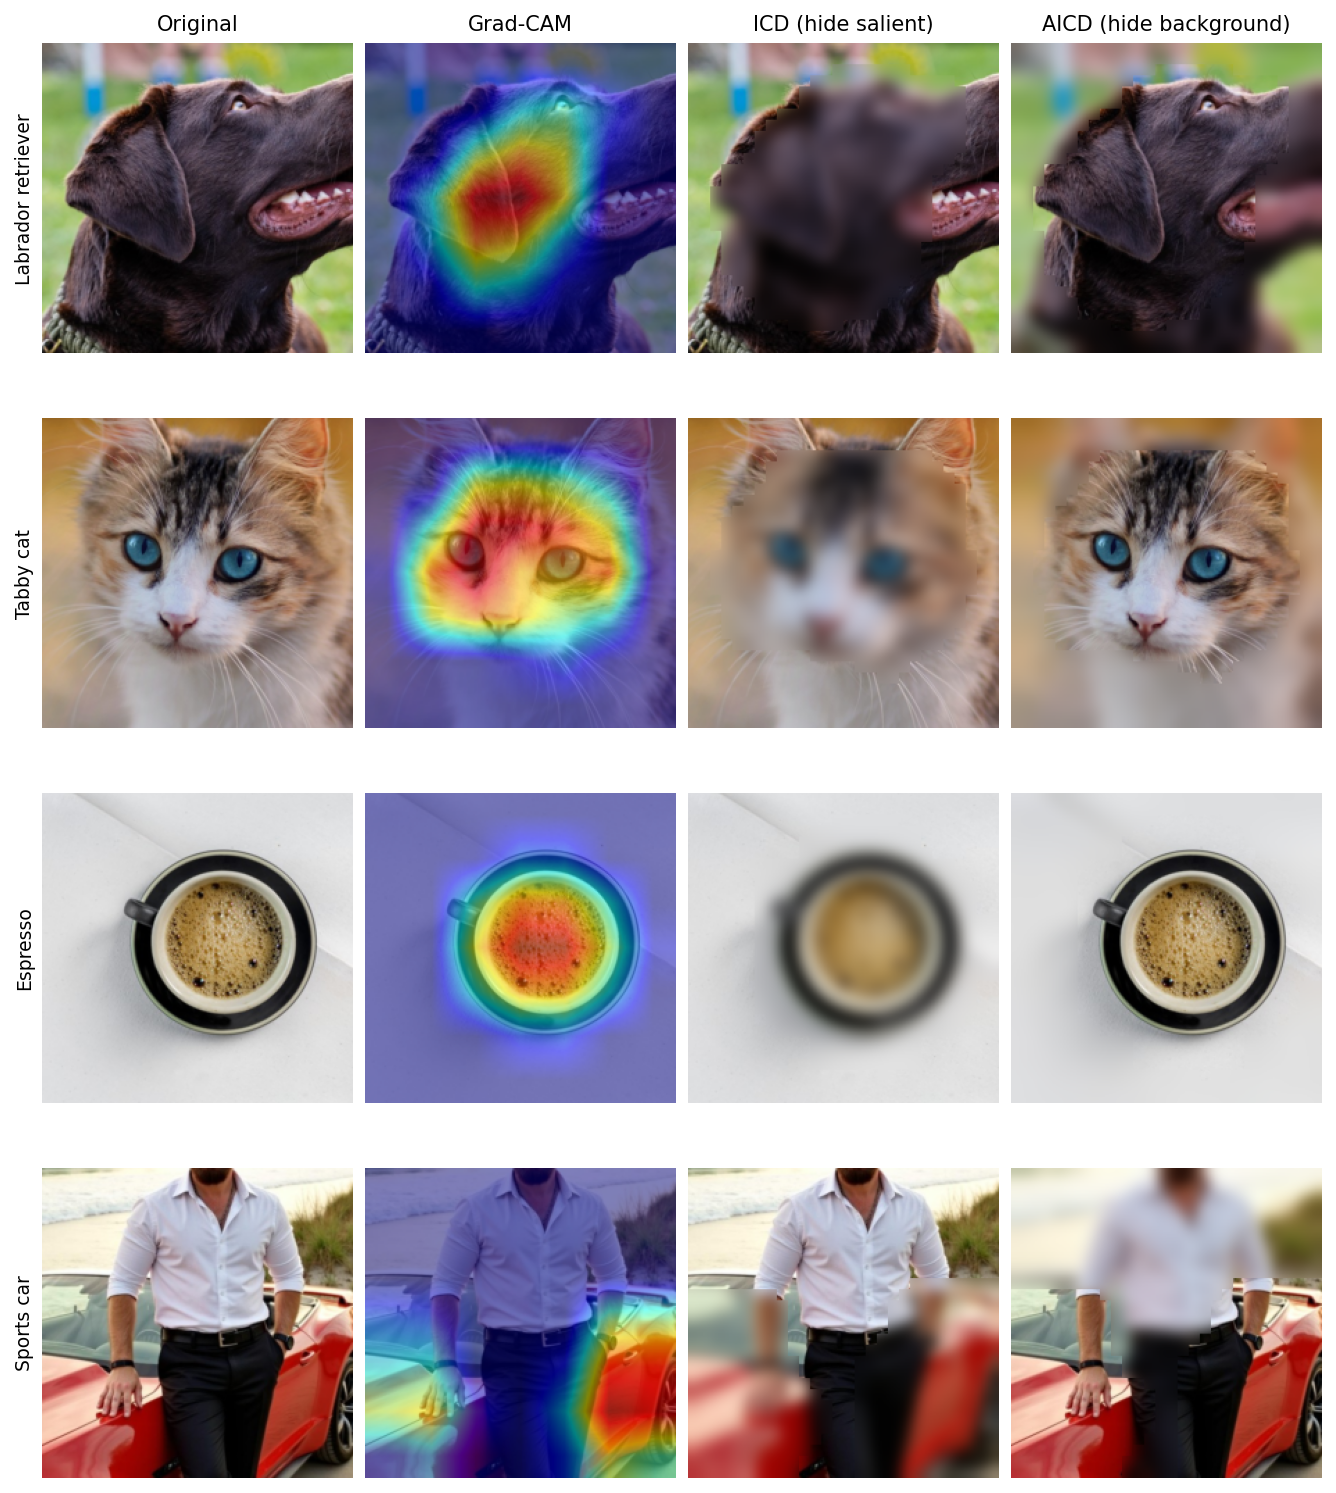
\includegraphics[width=0.72\linewidth]{figures/icd_aicd_comparison.png}
\caption{The ICD/AICD construction on four ImageNet classes.  From left to
right: the original image; the GradCAM saliency map at the final convolutional
layer of a ResNet-18; ICD, which masks the highest-saliency tiles
(Eq.~\ref{eq:icdmask}); and AICD, which masks the lowest-saliency tiles
(Eq.~\ref{eq:aicdmask}).  Both use $\rho = 0.5$ for clear visualisation and a
Gaussian-blur fill.  The same saliency map produces both masks.}
\label{fig:comparison}
\end{figure}

Figure~\ref{fig:fills} fixes the mask and varies the fill, illustrating the
qualitative difference between the strategies of Table~\ref{tab:fills} for both
ICD (top) and AICD (bottom).  Figure~\ref{fig:tiles} varies the tile size $t$:
small tiles trace the saliency contour closely but fragment the occlusion,
whereas large tiles produce a coarse, block-structured mask that is less
sensitive to saliency noise.

\begin{figure}[ht]
\centering
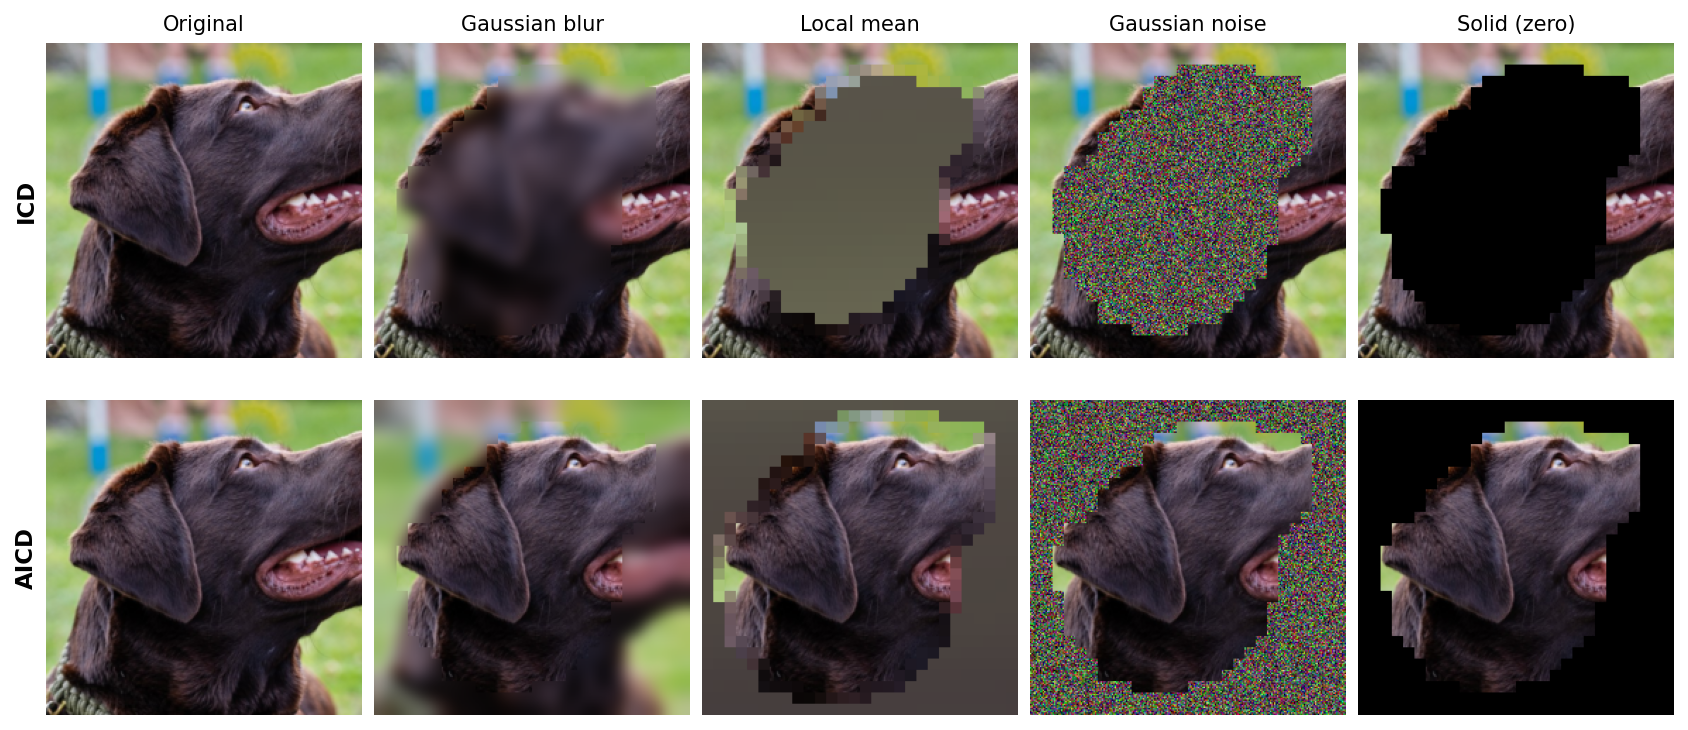
\includegraphics[width=0.92\linewidth]{figures/fill_strategies.png}
\caption{Four of the five fill strategies of Table~\ref{tab:fills} (the
\texttt{global\_mean} strategy is omitted for space) applied under a fixed mask,
for ICD (top row) and AICD (bottom row) on the same image.  Gaussian blur is the
default soft fill; local mean and noise preserve different aspects of the
original content; solid zero-fill is the hard limit and reduces to classical
Cutout.}
\label{fig:fills}
\end{figure}

\begin{figure}[ht]
\centering
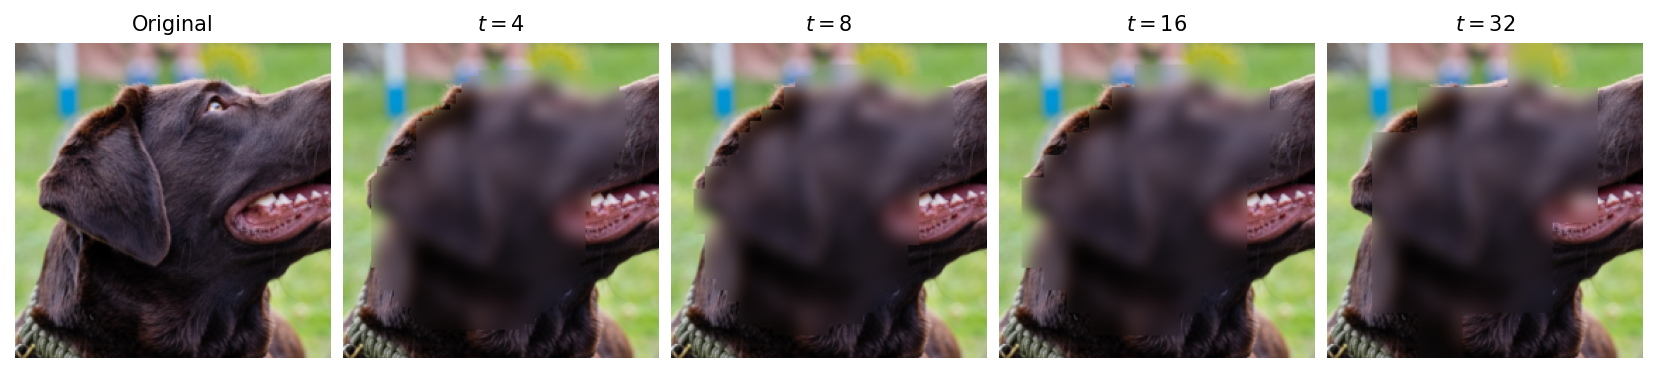
\includegraphics[width=0.92\linewidth]{figures/tile_sizes.png}
\caption{Effect of the tile size $t$ on the ICD mask (Gaussian-blur fill,
$\rho = 0.5$).  Smaller tiles follow the saliency map more closely at the cost
of a fragmented occlusion; larger tiles yield a coarser, more contiguous mask.}
\label{fig:tiles}
\end{figure}

\subsection{Hyperparameters}
\label{sec:method:hparams}

The construction has three principal hyperparameters.  The percentile $\rho$
sets the masked fraction $1-\rho$: larger $\rho$ masks fewer, more selective
tiles.  The tile size $t$ trades spatial fidelity for robustness, as in
Figure~\ref{fig:tiles}.  The fill $\phi$ determines what the network sees in
place of the occluded content.  In addition, each augmentation is applied
stochastically with probability $p$ per image, returning the image unchanged
with probability $1-p$; this keeps a fraction of clean images in every batch.
The library defaults are $t = 8$, Gaussian-blur fill, and a percentile of
$\rho = 0.70$; we set $p = 0.5$ for training so that half of each batch is
clean.  A lower $\rho$ is used only for the visualisations in this paper, where
a larger masked area is easier to read.

\FloatBarrier
